\chapter{Исследовательская часть}

В данном разделе будут приведены примеры работы программы, а также проведен сравнительный анализ процессорного времени и затрачиваемой памяти работы реализаций алгоритмов при различных ситуациях на основе полученных данных.

\section{Технические характеристики}

Технические характеристики устройства, на котором выполнялись замеры времени представлены далее:

\begin{itemize}
	\item операционная система Windows 11 Pro Версия 22H2 (22621.674) \cite{wind};
	\item память 16 ГБ;
	\item процессор 11th Gen Intel(R) Core(TM) i5-11400 2.59 ГГц \cite{proc}.
\end{itemize}

При тестировании компьютер был включен в сеть электропитания. Во время замеров процессорного времени устройство было нагружено только встроенными приложениями окружения, а также системой тестирования.

\section{Демонстрация работы программы}

На рисунке \ref{img:res} представлен результат работы программы. На экран выводятся результаты заемров времени для разных размеров строк и разных видов алгоритмов поиска расстояний Левенштейна и Дамерау-Левенштейна в мс.
\newpage
%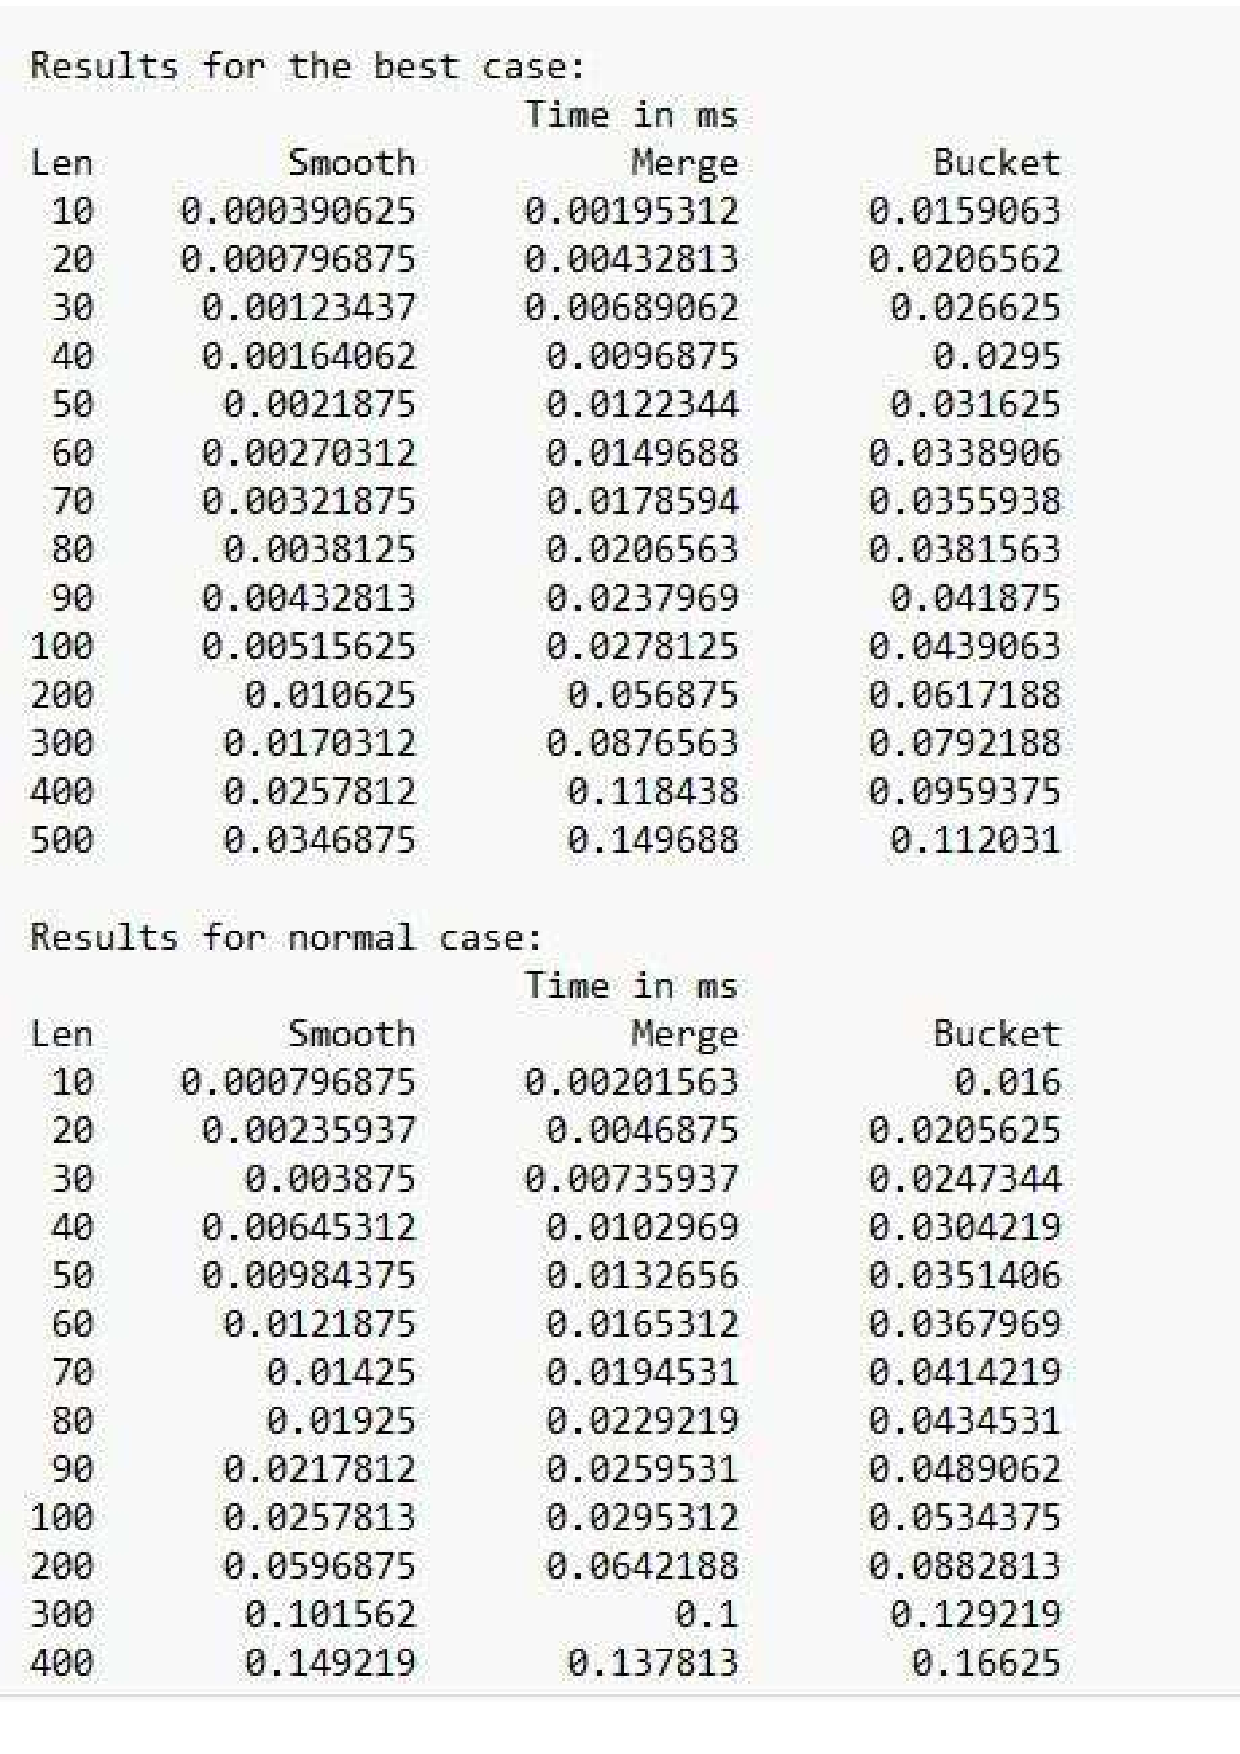
\includepdf[pages=-]{src/screen.pdf}
\begin{center}
	%\centering{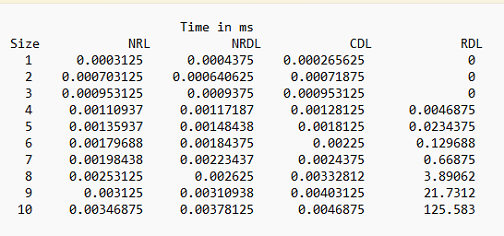
\includegraphics[trim=0 0 0cm 0cm bb=0 0 504 320]{src/screen}}
	\captionof{figure}{Пример работы программы}
	\label{img:res}
\end{center}

\section{Время выполнения реализаций алгоритмов}

Как было сказано выше, используется функция замера процессорного времени GetProcessTimes(...) из библиотеки Windows.h. 

\textbf{Входные данные:} строки размером от 10 до 500 элементов.

Результаты замеров времени работы реализаций алгоритмов поиска расстояний Левенштейна и Дамерау-Левенштейна на различных входных данных (в мс) приведены в таблице \ref{tbl:best}.


\begin{center}
	\begin{threeparttable}
		\caption{Процессорное время работы реализаций алгоритмов}
		\label{tbl:best}
		\begin{tabular}{|c|c|c|c|c|}
			\hline
			Размер & Л.(матр.) &  Д-Л.(матр.)  &  Д-Л.(рек.)& Д-Л.(рек. с кешем)\\
			\hline
			10 & 0  &  0.015625 &0 & \\ 
			\hline
		
		\end{tabular}
		
	\end{threeparttable}
\end{center}
Также на рисунке \ref{img:graph_sorted} приведены графические результаты замеров времени работы алгоритмов в зависимости от линейного размера входных строк.

\begin{center}
%	\centering{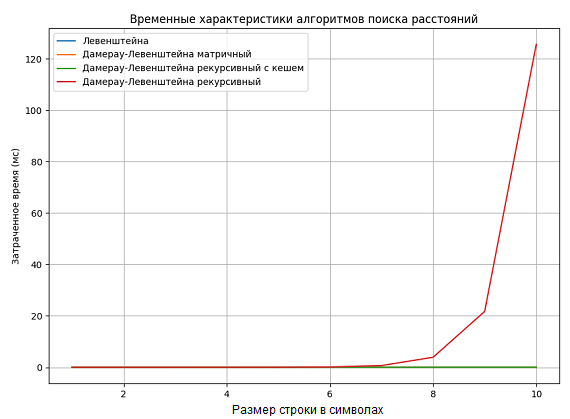
\includegraphics[trim=0 0 0 -5cm bb=0 0 570 650]{src/Graph}}
	\captionof{figure}{Процессорное время вычислений}
	\label{img:graph_sorted}
\end{center}
\newpage

\section{Затрачиваемая память при выполнении реализаций алгоритмов}

\section{Вывод}
%\addcontentsline{toc}{section}{Вывод}
